\chapter{Auswirkungen}
\label{chapter:auswirkungen}


\section{Prävalenz}

\section{Motivation}

Das primäre Motiv von Cyber-Kriminellen ist finanziell. Im Durchschnitt richtet ein 'Data Breach'
4.45 Millionen US-Dollar an Schaden an, wobei Social Engineering als initialer Angriffsvektor noch
über diesem Wert liegt \bcite{6_ibmsecurity}.


Der Verlust, nach erfolgreichen Social Engineering Angriffen, ist jedoch für Unternehmen weitreichender.
Neben dem direkten finanziellen Verlust, durch den Diebstahl der Angreifer erleiden Unternehmen zusätzlich
Wiederherstellungskosten, da etwaige Daten verloren gegangen sind, und Sicherheitslücken gefunden und repariert
werden müssen. Des Weiteren entsteht eine Betriebsdisruption, was zu indirektem finanziellen Schaden, durch
Verlust von Produktivität, führt. Zuletzt erleiden Unternehmen einen Reputationsschaden, was in vielen Fällen
den verheerendsten Faktor ausmacht, insbesondere für kleinere Firmen \bcite{agony}.
Für Unternehmen können Cyber-Angriffe auch eine Form der Espionage darstellen, weshalb der Schaden eines
Unternehmens zusätzlich einen kompetitiven Schaden in der Marktwirtschaft darstellen kann.

Individuen erleiden ebenfalls, neben finanziellen-, auch weitere Formen von Schäden.
Nicht außer Acht zu lassen ist der emotionale Schaden, da Personen oft, in Folge einer erfolgreichen
Manipulation, als naiv dargestellt werden.



% The median time for
% users to fall for phishing emails
% is less than 60 seconds. "\cite{verizon2024}


% \begin{figure}[H]
%     \centering
%     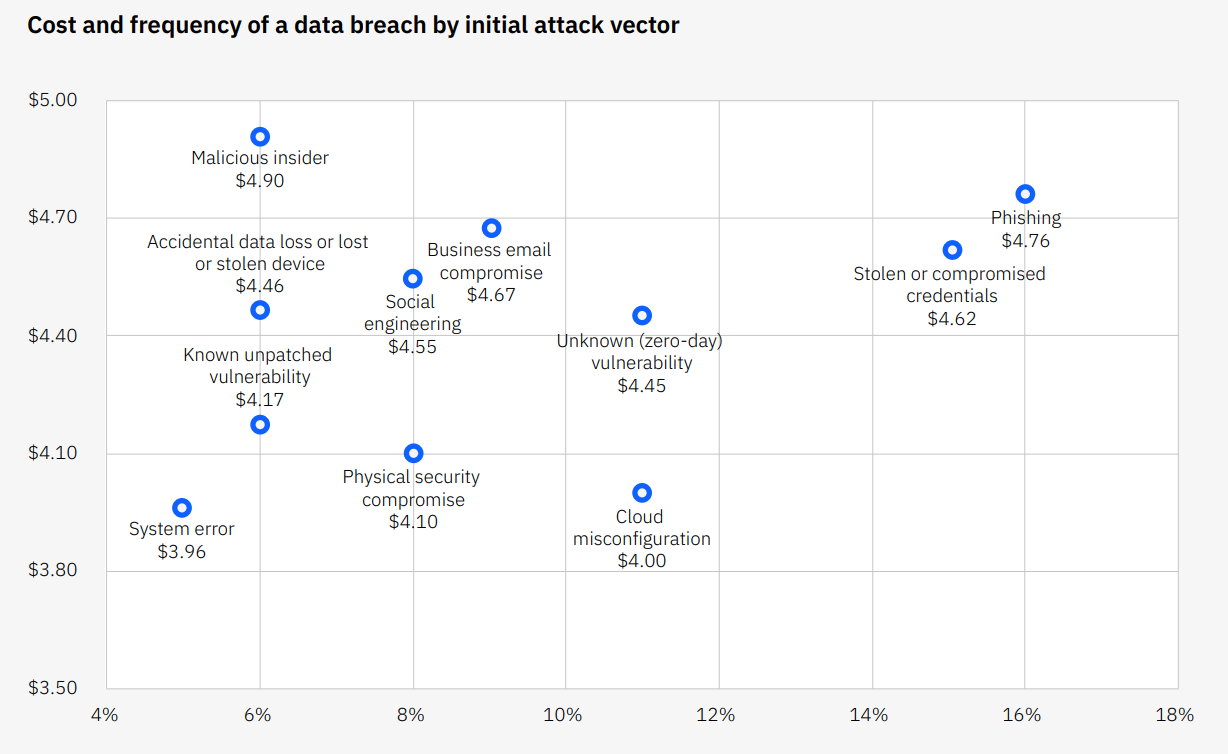
\includegraphics[width=5in]{IBM_Data.Breach.Report.png}
%     \caption{IBM - Measured in USD millions}
% \end{figure}
% Avg. Kosten pro Breach (2022)


% \begin{figure}[H]
%     \centering
%     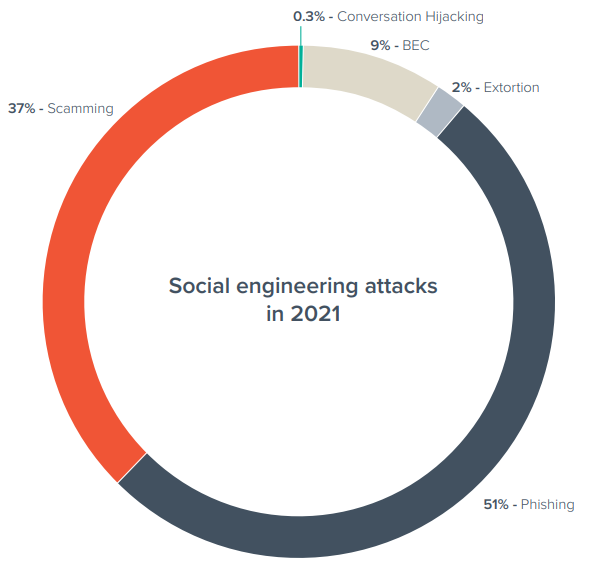
\includegraphics[scale=.5]{Barracuda_Social.Engineering.Attacks.png}
%     \caption{Barracuda - Social Engineering Attacks}
% \end{figure}


% \newpage

% "Actor Motives Financial (89\%), Espionage (11\%) (breaches)"\cite{verizon2022}
% "Actor Motives Financial (95\%), Espionage (5\%) (breaches)"\cite{verizon2024}

% conversation hijacking wenig ,denn verlangt etwas erfolg bei vorherigen angriffen.
% z.b. folgt onversation hijacking oftmals auf account takeover.

% "Hackers are starting to increasingly use phishing as part of their
% ransomware attacks."\cite{3_barracuda}

% "Extortion attacks make up only 2\% of the total number of
% targeted phishing attacks we have seen in the past year. These
% attacks were mostly sextortion email threats, where hackers
% threaten to expose sensitive or embarrassing content to their
% victim’s contacts unless a ransom is paid. Demands are usually
% a few hundred or a few thousand dollars and need to be paid
% in bitcoin, which is difficult to trace. In the UK, the number of
% sextortion cases reported to National Crime Agency increased
% by 88\% between 2018 and 2020, and the number is expected to
% continue to increase"\cite{3_barracuda} stand 2021
% stand 2024: Extortion: ($\sim$ 25\%) \cite{verizon2024}
% Darunter fällt auch Ransomware

% Pretexting: 2022 (27\%), 2024 (more than 40\%)
% Phishing: 2022 ($\sim$ 70\%), 2024 (31\%)\cite{verizon2024,verizon2022}

% "Account takeover is a form of identity theft and fraud where a
% malicious third party successfully gains access to a user’s account
% credentials"\cite{3_barracuda}
% "Account takeover is one of the fastest growing threats. In 2021,
% roughly 1 in 5 organizations (20\%) had at least one of their
% Microsoft 365 accounts compromised. This means that in 2021
% hackers managed to compromise around 500,000 Microsoft 365
% accounts around the globe."\cite{3_barracuda}

% Social Engineering MTTI (Mean Time To Identify): 218 Days
% Social Engineering MTTC (Mean Time To Contain) :  80 Days\cite{6_ibmsecurity}
